\subsection{Problema a resolver}


\subsection{Resolución coloquial}


\subsection{Demostración de correctitud}

Primero veamos el invariante de nuesta solucion:
\begin{itemize}
\item Sea S una solucion, cumple que el i-esimo curso tiene la fecha de finalizacion mas proxima posible\footnote{Con "posible" nos referimos a que no se solapa con ningun curso que tenga menor fecha de finalizacion.} al anterior, es decir, al (i-1)-esimo curso. Estando siempre el curso que primero finaliza como solucion.
\end{itemize}

Sea C un conjunto de cursos tal que:
\begin{itemize}
\item Ningun curso se solapa, la solucion es C. Esto es trivial, ya que mas cursos de los que hay no pueden  haber.
\item Existen dos cursos que se solapan. Sea $i$ y $j$ dichos cursos. Sin perder generalidad supongamos que la fecha de terminacion de $j$ es mayor o igual que la de $i$. Quiero ver que, si S es la solucion que contiene a $i$ y S' es la solucion que contiene a $j$ $\Rightarrow$ $|$S'$|$ $\leq$ $|$S$|$. 
  Esto se cumple porque S' contiene a $j$ que termina luego que $i$, por lo que por lo menos todos los cursos de S' desde el $j$ estan contenidos en S y, ademas, si  $j$ comienza antes que $i$ se que la cantidad de cursos de S' antes de $j$ estan antes de $i$ en S 

\begin{figure}[H] %[h] Aqui [b] para button [t] para top
\begin{center}
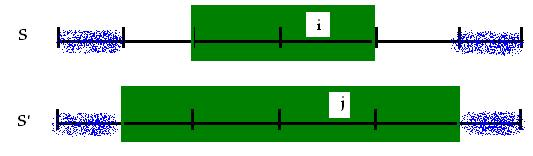
\includegraphics[width=322pt]{../imgs/demo21.jpg}
\end{center}
\end{figure}

ò si $j$ empieza luego de $i$ yo se que no termina ningun otro curso entre el comienzo de $i$ y $j$, porque de terminar ubiese elejido ese en S  (ya que elijo siempre el que termina antes), 

\begin{figure}[H] %[h] Aqui [b] para button [t] para top
\begin{center}
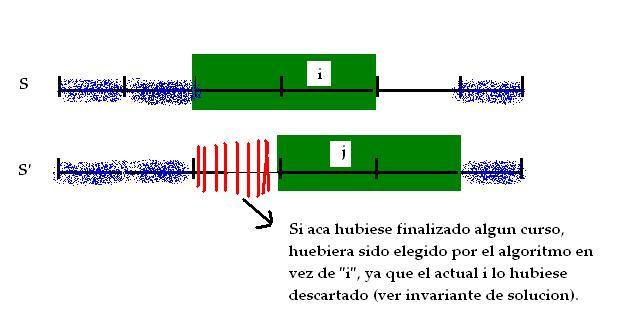
\includegraphics[width=322pt]{../imgs/demo22.jpg}
\end{center}
\end{figure}

\end{itemize}

por lo tanto, $|$S'$|$ $\leq$ $|$S$|$. 


\subsection{Complejidad del algoritmo}

\subsection{Código fuente}



\subsection{Instancias posibles}



\subsection{Testing}